%appendix D
%mac

%\section{Process: MAC}

\section{Overview}
\begin{figure}[ht]
    \centering
    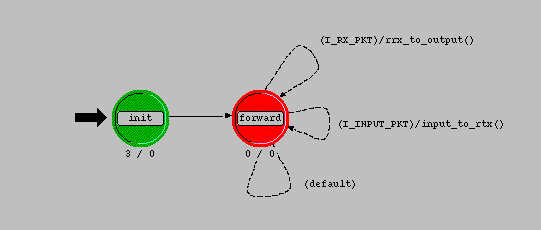
\includegraphics[width=.7\textwidth]{images/mac}
    \caption{MAC process model}
    \label{fig:appendix-d}
\end{figure}

\newpage

\section{Local variables}
\begin{figure}[ht]
    \centering
    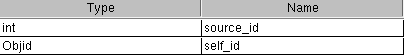
\includegraphics[width=.7\textwidth]{images/state_variable_mac}
    \caption{State variables of MAC process}
    \label{fig:appendix-d_sv}
\end{figure}

\section{Header Block}
%_____________________________________HEADER______________________________________
{\tiny
\begin{verbatim}
//Streams
#define STRM_INPUT		0
#define STRM_RRX		1
#define STRM_OUTPUT 	0
#define STRM_RTX		1
//Interrupts
#define I_RX_PKT		(op_intrpt_type() == OPC_INTRPT_STRM && op_intrpt_strm() == STRM_RRX)
#define I_INPUT_PKT		(op_intrpt_type() == OPC_INTRPT_STRM && op_intrpt_strm() == STRM_INPUT)
void rrx_to_output(void);
void input_to_rtx(void);

\end{verbatim}
}

\section{Function Block}
%______________________________FUNCTION__________________________________
{\tiny
\begin{verbatim}

void rrx_to_output(void)
{
	Packet *pPkt;
	Objid pktsource;
	char message_str[255];
	FIN(rrx_to_output());
	pPkt = op_pk_get(STRM_RRX);
	op_pk_nfd_get(pPkt, "mac_source", &pktsource);
	if(pktsource == self_id)
	{		
		op_pk_destroy(pPkt);
	}
	else
	{
		op_pk_send(pPkt, STRM_OUTPUT);
	}
	FOUT;
}
void input_to_rtx(void)
{
	Packet *pPkt;
	FIN(input_to_rtx());
	pPkt = op_pk_get(STRM_INPUT);
	op_pk_nfd_set_objid(pPkt, "mac_source", self_id);
	op_pk_send(pPkt, STRM_RTX);
	FOUT;
}

\end{verbatim}
}

\section{init State: Enter Executives}
%______________________________________Init_____________________________________________________________
{\tiny
\begin{verbatim}
self_id = op_id_self();
op_ima_obj_attr_get (self_id, "Source ID", &source_id);

\end{verbatim}
}
